\documentclass[12pt,letterpaper]{article}
\usepackage[utf8]{inputenc}
\usepackage[spanish]{babel}
\usepackage{graphicx}
\usepackage[left=2cm,right=2cm,top=2cm,bottom=2cm]{geometry}
\usepackage{graphicx} % figuras
% \usepackage{subfigure} % subfiguras
\usepackage{float} % para usar [H]
\usepackage{amsmath}
%\usepackage{txfonts}
\usepackage{stackrel} 
\usepackage{multirow}
\usepackage{enumerate} % enumerados
\renewcommand{\labelitemi}{$-$}
\renewcommand{\labelitemii}{$\cdot$}
% \author{}
% \title{Caratula}
\begin{document}

% Fancy Header and Footer
% \usepackage{fancyhdr}
% \pagestyle{fancy}
% \cfoot{}
% \rfoot{\thepage}
%

% \usepackage[hidelinks]{hyperref} % CREA HYPERVINCULOS EN INDICE

% \author{}
\title{Caratula}

\begin{titlepage}
\begin{center}
\large{UNIVERSIDAD PRIVADA DE TACNA}\\
\vspace*{-0.025in}
\begin{figure}[htb]
\begin{center}

\includegraphics[width=8cm]{./Imagenes/logo}
\end{center}
\end{figure}
\vspace*{0.15in}
INGENIERIA DE SISTEMAS  \\

\vspace*{0.5in}
\begin{large}
TITULO:\\
\end{large}

\vspace*{0.1in}
\begin{Large}
\textbf{TRABAJO DE INVESTIGACION ACERCA DE GITHUB Y SIMILARES} \\
\end{Large}

\vspace*{0.3in}
\begin{Large}
\textbf{CURSO:} \\
\end{Large}

\vspace*{0.1in}
\begin{large}
BASE DE DATOS II\\
\end{large}

\vspace*{0.3in}
\begin{Large}
\textbf{DOCENTE(ING):} \\
\end{Large}

\vspace*{0.1in}
\begin{large}
 Patrick Cuadros Quiroga\\
\end{large}

\vspace*{0.2in}
\vspace*{0.1in}
\begin{large}
Alumna: \\
\begin{flushleft}
Leydi Katherine Huallpa Castro	           \hfill	(2015053230) \\
\end{flushleft}
\end{large}

\vspace*{0.3in}
\begin{Large}
\textbf{TACNA-PERU:} \\
\end{Large}

\vspace*{0.1in}
\begin{large}
2018\\
\end{large}

\end{center}

\end{titlepage}


\part{Introduccion a GITHUB}

\section{¿Que es Github?}
Github es una plataforma creada para facilitar el desarrollo colaborativo de software, nos permite alojar proyectos en la web gratuitamente, por lo general de forma pública, aunque podemos alojar los proyectos de modo privado, si pagamos una pequeña suscripción mensual.

\vspace*{-0.025in}
\begin{figure}[htb]
\begin{center}

\includegraphics[width=8cm]{./Imagenes/Git}
\end{center}
\end{figure}

\section{¿Para que sirve?}
GitHub aloja tu repositorio de código y te brinda herramientas muy útiles para el trabajo en equipo, dentro de un proyecto.

\vspace*{-0.025in}
\begin{figure}[htb]
\begin{center}

\includegraphics[width=8cm]{./Imagenes/herramienta-tee}
\end{center}
\end{figure}

Además de eso, puedes contribuir a mejorar el software de los demás. Para poder alcanzar esta meta, GitHub provee de funcionalidades para hacer un fork y solicitar pulls.

\vspace*{-0.025in}
\begin{figure}[htb]
\begin{center}

\includegraphics[width=8cm]{./Imagenes/colaboracion}
\end{center}
\end{figure}

Realizar un fork es simplemente clonar un repositorio ajeno (genera una copia en tu cuenta), para eliminar algún bug o modificar cosas de él. Una vez realizadas tus modificaciones puedes enviar un pull al dueño del proyecto. Éste podrá analizar los cambios que has realizado fácilmente, y si considera interesante tu contribución, adjuntarlo con el repositorio original.

\vspace*{-0.025in}

\section{¿Que herramientas proporciona?}
En la actualidad, GitHub es mucho más que un servicio de alojamiento de código. Además de éste, se ofrecen varias herramientas útiles para el trabajo en equipo. Entre ellas, caben destacar:

\begin{itemize}
    \item Un sistema de seguimiento de problemas que permiten a los miembros de tu equipo detallar un problema con tu software o una sugerencia que deseen hacer.
    \item Una herramienta de revisión de código, donde se pueden añadir anotaciones en cualquier punto de un fichero y debatir sobre determinados cambios realizados en un commit específico.
    \item Un visor de ramas donde se pueden comparar los progresos realizados en las distintas ramas de nuestro repositorio.
\end{itemize}

\vspace*{-0.025in}
\begin{figure}[htb]
\begin{center}

\includegraphics[width=8cm]{./Imagenes/trabajo-en-equipo}
\end{center}
\end{figure}

\part{5 Mejores alternativas a GITHUB}

\section{GITLAB}
Sin duda una de las mejores alternativas, GitLab es un servicio web de código abierto, potente, seguro, eficiente en funciones y sólido para el control de versiones y desarrollo de software colaborativo basado en Git. Además de gestor de repositorios, el servicio ofrece también alojamiento de wikis y un sistema de seguimiento de errores.
Admite hitos de grupo, rastreador de problemas, tableros de problemas configurables y problemas de grupo, traslado de problemas entre proyectos y más.
También cuenta con potentes herramientas de bifurcación, ramas y etiquetas protegidas, bloqueo de archivos, solicitudes de fusión, notificaciones personalizadas, hojas de ruta del proyecto, problemas de ponderación, cuestiones confidenciales y relacionadas, gráficos burndown para hitos del proyecto y del grupo.

\vspace*{-0.025in}
\begin{figure}[htb]
\begin{center}
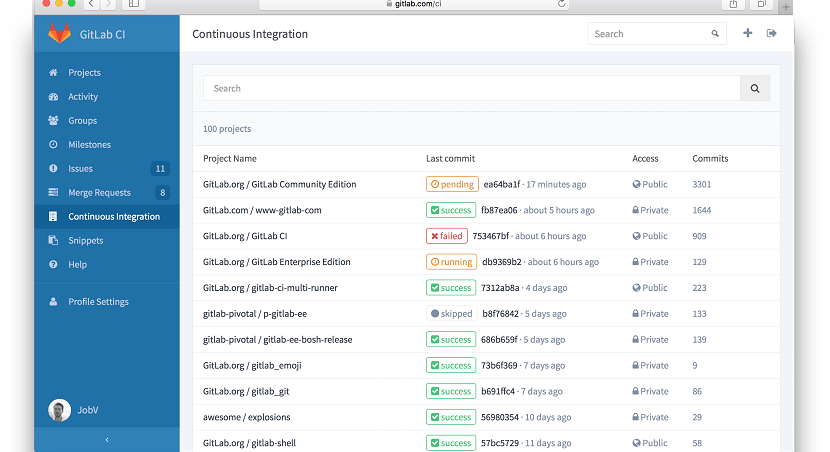
\includegraphics[width=16cm]{./Imagenes/gitlab}
\end{center}
\end{figure}

\section{GOGS}
Gogs es un servicio gratuito de código abierto está disponible bajo la Licencia MIT es bastante ligero y multiplataforma se ejecuta en cualquier lugar donde Go pueda compilar para: Windows, Mac, Linux, ARM, etc.
Es fácil de instalar y lo suficientemente pequeño para ejecutarse en una Raspberry Pi. Gogs es probablemente la forma más fácil y rápida de configurar su propia solución de hosting de código alojado.

\begin{figure}[htb]
\begin{center}
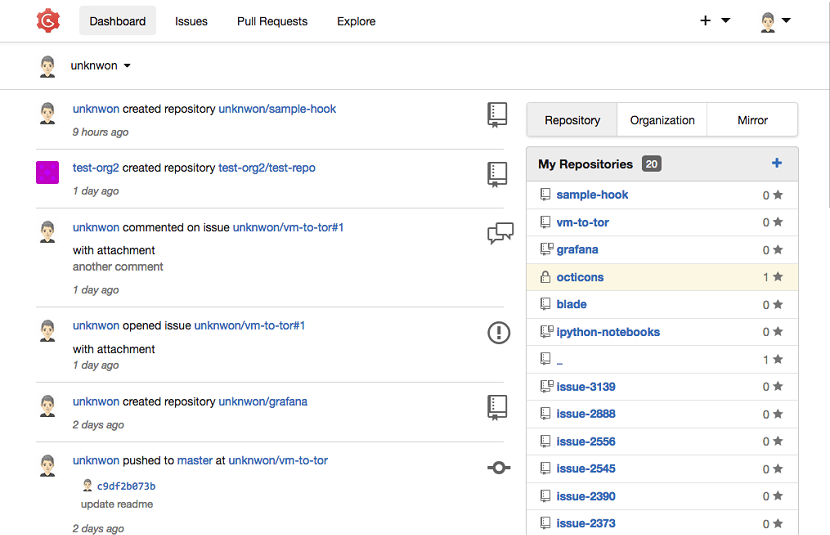
\includegraphics[width=8cm]{./Imagenes/gogs}
\end{center}
\end{figure}

\section{GITEA}
Gitea es una bifurcación gestionada por la comunidad de Gogs, el servicio de Gitea de Git auto hospedado es totalmente gratuito. Esta es una solución de alojamiento de código liviano escrita en Go y publicada bajo la licencia MIT.
También es un método simple y rápido de configurar un servicio de Git auto hospedado para el desarrollo de software de código abierto.

\vspace*{-0.025in}
\begin{figure}[htb]
\begin{center}
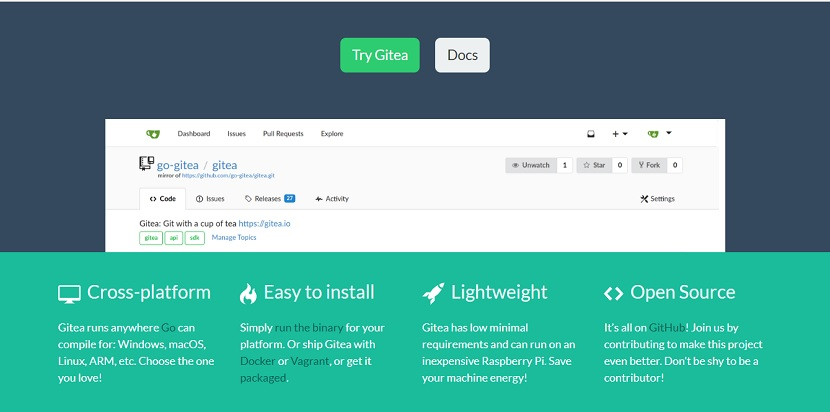
\includegraphics[width=16cm]{./Imagenes/gitea}
\end{center}
\end{figure}

\section{BITBUCKET}
Bitbucket es un servicio de alojamiento basado en web, para los proyectos que utilizan el sistema de control de versiones Mercurial y Git. Bitbucket ofrece planes comerciales y gratuitos.
Bitbucket cuenta con bastantes características notables tales como la búsqueda de código, las solicitudes de extracción, cuenta con modelos de implementación flexibles, visualización de diferencias, la creación de reflejos inteligente, el seguimiento de problemas se puede configurar en el listas blancas de IP y permisos de sucursales para salvaguardar su flujo de trabajo.

\vspace*{-0.025in}
\begin{figure}[htb]
\begin{center}
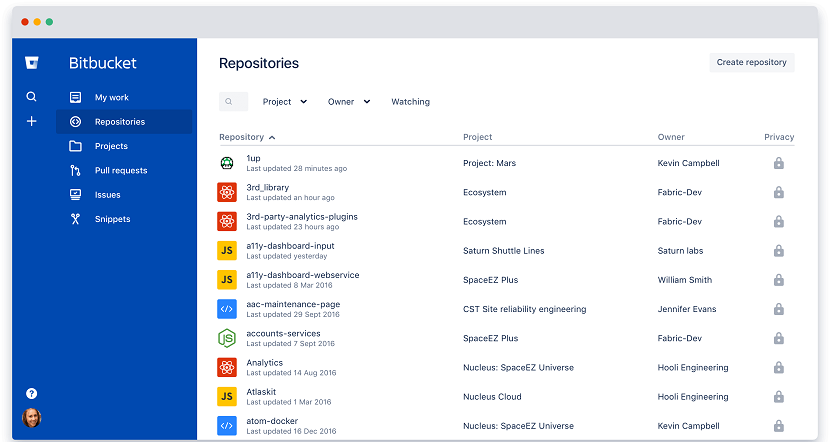
\includegraphics[width=8cm]{./Imagenes/bitbucket}
\end{center}
\end{figure}

\section{BEANSTALK}
Beanstalk es una plataforma potente, segura, de alto rendimiento y confiable para administrar repositorios de código fuente.
Beanstalk está diseñado para mejorar su flujo de trabajo de desarrollo utilizando funciones como las solicitudes de revisión de código, rastreador de problemas, también se cuenta con las estadísticas de repositorio, las notas de la versión, las notificaciones, los resúmenes de correo electrónico, vista de comparación, un historial completo de confirmaciones y archivos y mucho más.

\vspace*{-0.025in}
\begin{figure}[htb]
\begin{center}
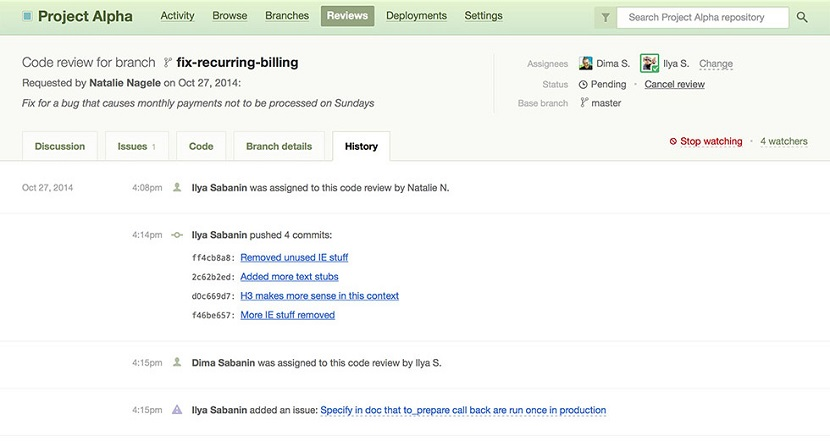
\includegraphics[width=16cm]{./Imagenes/beanssaltk}
\end{center}
\end{figure}

\end{document}
